\subsection{{Etapas de funcionamento do sistema}}

O funcionamento da ferramenta consiste em analisar uma imagem de um jogador objetivando adquirir todos os pontos de interesse da imagem, que servirá como parâmetro de busca para que o algoritmo seja mais eficiente quando o mesmo for exposto a uma situação mais complexa como por exemplo, analisar um jogador com capacete.

A análise feita pelo algoritmo ocorre de forma minuciosa e utilizando técnicas de processamento de imagem. Sendo assim, após a extração de todos os pontos de interesse da imagem, o algoritmo monta um conjunto de sequências lógicas das taxas de \textit{pixels} existentes nesses pontos. Esta conversão pode ser demostrada de forma mais clara na \autoref{fig_conversao_img} da \autoref{descricao-do-sistema}.

Após a montagem do conjunto, o algoritmo utiliza um dispositivo de captura de imagem para realizar uma busca por similaridade, ou seja, o algoritmo buscará algo semelhante ao padrão montado na etapa anterior. Após a busca feita pelo \textit{software}, a detecção vai definir se existe ou não um jogador no ambiente que está sendo analisado. Se for constatado que existe um jogador e ele for igual ao modelo, a ferramenta vai apresentar o seu nome cadastrado. A \autoref{fig_fluxograma_proj} representa o fluxograma do \textit{software}.

\begin{figure}[h]
	\caption{\label{fig_fluxograma_proj}Fluxograma de funcionamento do sistema.}
	\begin{center}
		\resizebox{.9\linewidth}{!}{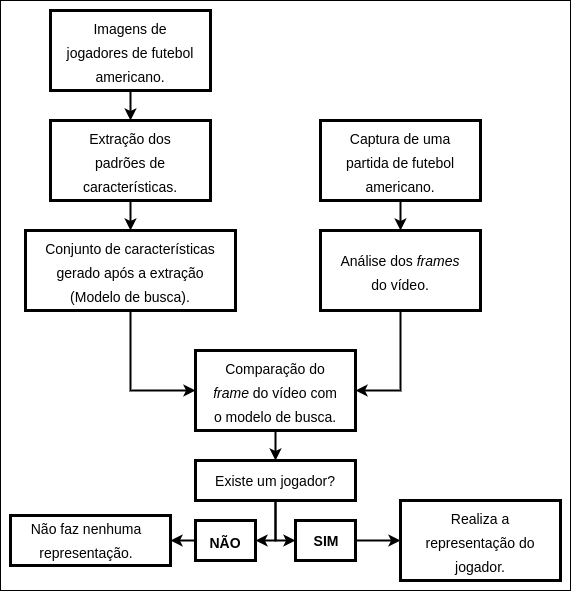
\includegraphics{6-Desenvolvimento-Projeto/imagens-desenvolvimento/fluxograma-projeto.png}}
	\end{center}
	\centering \legend{Fonte: Elaborada pelos autores.}
\end{figure}

Ao final do processo, será feito uma análise dos dados apresentados pela ferramenta. Através desses dados, pode-se obter o percentual de acertos e erros, analisando também os cenários de maior e menor eficiência.